\documentclass[12pt]{article}

\usepackage[utf8]{inputenc}
\usepackage[OT1]{fontenc}
\usepackage{graphicx}
\usepackage[frenchb]{babel}
\usepackage{multirow}
\usepackage{hyperref}

\hypersetup{
    colorlinks,
    citecolor=black,
    filecolor=black,
    linkcolor=black,
    urlcolor=black
}

\usepackage{geometry}

\begin{document}
\thispagestyle{empty}
    \begin{center}
        \begin{figure}[h]
            \centering
            
\includegraphics[width=0.7\textwidth]{Logo_UT3.jpg}
        \end{figure}
        \Huge \textbf{R A P P O R T} \normalsize\\\vfill
        \emph{Ce rapport est réalisé par}\\
        \Large Khalil MAACHOU\\
        \rule{0.8\textwidth}{2pt}\\
        \huge\fontfamily{lmr}\selectfont TP meta-heuristique\\
        \LARGE Voyageur de commerce\\
        \rule{0.8\textwidth}{2pt}\\
        \begin{figure}[h]
            \centering
            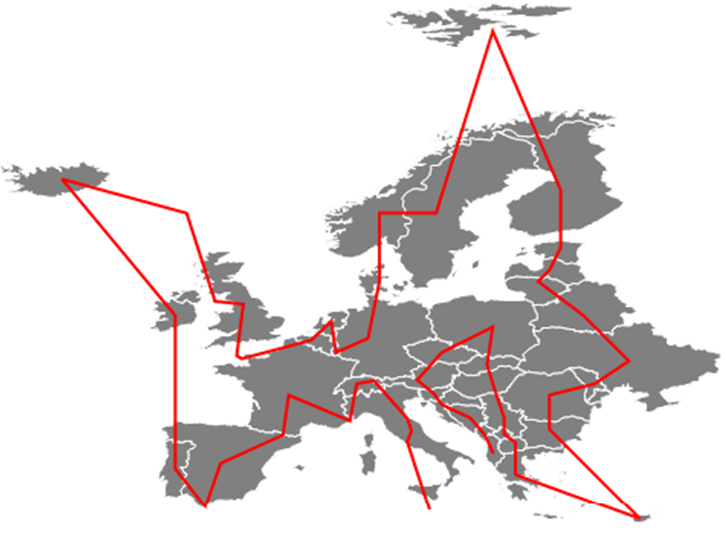
\includegraphics[width=0.5\textwidth]{TSP.png}
        \end{figure}
    \end{center}
    \begin{center}
        \begin{tabular}{lll}
            \hline\hline
            \emph\Large {Résponsable de Tp} & \Large trong-hieu tran & \Large Trong-Hieu.Tran@irit.fr \\ 
            \hline\hline
        \end{tabular}
    \end{center}
    \begin{center}
        \emph{2022/2023}
    \end{center}

    \newpage
        \tableofcontents
    \newpage
        \section{Introduction du probleme TSP}
        Le problème du voyageur de commerce (TSP pour Travelling Salesman Problem) est un problème de programmation linéaire qui consiste à trouver un circuit de longueur minimale passant par un certain nombre de villes données, en visitant chaque ville une seule fois avant de retourner à la ville de départ.

        Le TSP est un problème NP-difficile, ce qui signifie qu'il n'existe pas de méthode algorithmique efficace pour trouver la solution optimale de manière générale. Cependant, il existe de nombreuses heuristiques (algorithmes qui ne garantissent pas de trouver la solution optimale mais qui sont souvent très performants en pratique) qui permettent de trouver des solutions de qualité pour des instances de taille raisonnable.
        \section{Algorithmes implementés}
                Le problème du voyageur de commerce (TSP) peut être résolu en utilisant la méthode d'escalade avec redémarrages. Dans ce cas, la fonction de coût est la distance totale parcourue par le voyageur de commerce visitant toutes les villes du circuit, en partant de la ville de départ et en revenant dans cette ville.

            \subsection{Hill climbing avec redemarrage}
                Pour utiliser le hill-climbing avec redémarrages pour résoudre le TSP, nous devons d'abord définir la représentation de la solution comme un vecteur de villes. Par exemple, si votre visite doit passer par les villes 1, 2, 3, 4 et 5 (le cas de 5 villes tsp5.txt), vous pouvez représenter la solution avec le vecteur [1, 2, 3, 4, 5].

                Ensuite, nous devons définir deux fonctions. L'un pour calculer le coût de la solution (en utilisant la distance euclidienne) et l'autre pour calculer le plus proche voisin à choisir s'il existe.

                Enfin, pour chaque iteration (nombre d'essaies) et à partir d'une solution aléatoire S à chaque itération on va répéter :

                \hspace{0.6cm}- Chercher le meilleur voisin V à partir de la solution S en utilisant la fonction meilleur voisin.

                \hspace{0.6cm}- Si V est meilleur que S alors en permute les deux et on répète sinon en termine notre hill climbing.

                \hspace{0.6cm}- Il existe deux conditions d'arrêt : soit y ont plus de voisins meilleurs ou on arrive au déplacement maximal.
                
                jusqu'à qu'on arrive au nombre d'essais maximals.\\
                
            \subsection{Tabou}
                Pour L'algorithme Tabou pour résoudre le TSP, nous devons d'abord  aussi définir la représentation de la solution comme un vecteur de villes. Par exemple, si votre visite doit passer par les villes 1, 2, 3, 4 et 5 (le cas de 5 villes tsp5.txt), vous pouvez représenter la solution avec le vecteur [1, 2, 3, 4, 5].

                Ensuite, il faut définir deux fonctions. Une pour calculer le coût de la solution (en utilisant la distance euclidienne) et l'autre pour calculer le plus proche voisin non tabou (défini dans la section d'avant) à choisir s'il existe.

                Enfin, à partir d'une solution aléatoire S  qui est considerer comme la valeur initiale mSol (meilleur solution) à chaque itération on va répéter :

                \hspace{0.6cm}- Chercher le meilleur voisin V à partir de la solution S en utilisant la fonction meilleur voisin non tabou.

                \hspace{0.6cm}- Si V est meilleur que mSol alors en permute les deux et dans tous les cas on affecte la valeur de voisin à S (S = V).

                \hspace{0.6cm}- Il existe deux conditions d'arrêt : soit y ont plus de voisins non Tabou ou on arrive au déplacement maximal.
                
                jusqu'à qu'on arrive au nombre de deplacement maximal ou y a plus de voisin non tabou disponible.\\
        \section{Voisinages implementés}
                Un voisin d'une solution S pour le problème TSP représente une permutation de deux villes par rapport à une solution S.

            \subsection{Meilleur voisin Hill climbing}
                Un meilleur voisin pour Hill climbing d'une solution S est un parcours de tous les voisins de S en choisissant celui avec la meilleur valeur (en cas de plusieurs on choisi un voisin aléatoirement).

            \subsection{Meilleur voisin non Tabou}
                Un meilleur voisin pour Tabou d'une solution S est un parcours de tous les voisins de S en choisissant celui avec la meilleur valeur et qui n'est pas inclus dans la liste tabou (en cas de plusieurs on choisi un voisin aléatoirement).

        \section{Testes / Résultats Hill climbing}
            Pour chaque cellule : 1ere ligne = valeur en KM, 2eme ligne = temps d'exec en seconds, 3eme ligne = nombre de déplacements effectuer. \\
            
            \subsection{TSP5}
            \begin{tabular}{|c|c|c|c|c|c|c|}
                \hline
                {Taille, Max Depl} & 10 & 15 & 40 & 80 &  150 & 500 \\
                \hline
                \multirow{4}{*}{3} & 194.0405 & 194.0405 & 194.0405 & 196.1247 & 194.0405 & 194.0405  \\ & 0.00428 & 0.00289 & 0.00333 & 0.00392 & 0.00258 & 0.00264  \\ & 0 & 1 & 2 & 3 & 1 & 1  \\\hline
                \multirow{4}{*}{5} & 194.0405 & 194.0405 & 194.0405 & 194.0405 & 194.0405 & 194.0405  \\ & 0.0039 & 0.00487 & 0.00597 & 0.00481 & 0.00446 & 0.00454  \\ & 1 & 2 & 3 & 2 & 2 & 1  \\\hline
                \multirow{4}{*}{10} & 194.0405 & 194.0405 & 194.0405 & 194.0405 & 194.0405 & 194.0405  \\ & 0.0097 & 0.00962 & 0.0084 & 0.00887 & 0.00917 & 0.0092  \\ & 2 & 2 & 2 & 2 & 3 & 2  \\\hline
                \multirow{4}{*}{50} & 194.0405 & 194.0405 & 194.0405 & 194.0405 & 194.0405 & 194.0405  \\ & 0.04771 & 0.05813 & 0.04727 & 0.04685 & 0.04225 & 0.04501  \\ & 2 & 2 & 2 & 1 & 1 & 1  \\\hline
                \multirow{4}{*}{100} & 194.0405 & 194.0405 & 194.0405 & 194.0405 & 194.0405 & 194.0405  \\ & 0.10416 & 0.08937 & 0.09529 & 0.09288 & 0.10301 & 0.09543  \\ & 2 & 2 & 2 & 3 & 2 & 2  \\\hline 
                \multirow{4}{*}{500} & 194.0405 & 194.0405 & 194.0405 & 194.0405 & 194.0405 & 194.0405  \\ & 0.473 & 0.47281 & 0.49058 & 0.47689 & 0.47525 & 0.49421  \\ & 3 & 3 & 2 & 2 & 2 & 2  \\\hline
            \end{tabular}
            \subsection{TSP101}
            \begin{tabular}{|c|c|c|c|c|c|}
                \hline
                {Essaie, Max Depl} & 10 & 15 & 40 & 80 & 150 \\ \hline
                \multirow{4}{*}{2} & 2862.6681 & 2534.9666 & 1725.1056 & 1378.9494 & 1172.0434  \\ & 2.1875 & 3.29688 & 9.26562 & 18.15625 & 26.625  \\ & 10 & 15 & 40 & 80 & 110  \\\hline
                \multirow{4}{*}{5} & 2869.3667 & 2500.6084 & 1648.9099 & 1379.6783 & 1196.9764  \\ & 4.3125 & 6.57812 & 17.79688 & 36.26562 & 52.60938  \\ & 10 & 15 & 40 & 80 & 116  \\\hline
                \multirow{4}{*}{10} & 2901.7191 & 2561.8696 & 1684.6938 & 1204.173 & 1176.8398  \\ & 6.82812 & 10.01562 & 27.51562 & 56.65625 & 88.54688  \\ & 10 & 15 & 40 & 80 & 126  \\\hline
                \multirow{4}{*}{30} & 2874.7306 & 2424.3701 & 1570.3484 & 1220.0016 & 1004.4198  \\ & 11.8125 & 17.14062 & 46.40625 & 92.125 & 135.54688  \\ & 10 & 15 & 40 & 80 & 141  \\\hline
            \end{tabular}
            \paragraph{Note :\\}
            J'ai fait l'ensemble des tests dans le tableau avec une machine (i7) vu que ma machine n'est pas assez performante pour l'instance avec 101 villes et c'est pour ça j'ai pas fait trop de tests avec des parametres trop grands.
        \section{Testes / Résultats Tabou}
            Pour chaque cellule : 1ere ligne = valeur en KM, 2eme ligne = temps d'exec en seconds, 3eme ligne = nombre de déplacements effectuer. \\

            \subsection{TSP5}
            \begin{tabular}{|c|c|c|c|c|c|c|}
                \hline
                {Taille, Max Depl} & 5 & 10 & 20 & 25 & 100 & 500 \\
                \hline
                \multirow{4}{*}{2} & 194.0405 & 194.0405 & 194.0405 & 194.0405 & 194.0405 & 194.0405  \\ & 0.01926 & 0.01531 & 0.03774 & 0.05552 & 0.10267 & 0.38383  \\ & 10 & 15 & 40 & 80 & 150 & 500  \\\hline
                \multirow{4}{*}{5} & 194.0405 & 194.0405 & 194.0405 & 194.0405 & 194.0405 & 194.0405  \\ & 0.00785 & 0.01212 & 0.03287 & 0.06582 & 0.12471 & 0.42561  \\ & 10 & 15 & 40 & 80 & 150 & 500  \\\hline
                \multirow{4}{*}{10} & 194.0405 & 194.0405 & 194.0405 & 194.0405 & 194.0405 & 194.0405  \\ & 0.00844 & 0.01317 & 0.04062 & 0.07885 & 0.19113 & 0.56123  \\ & 10 & 15 & 40 & 80 & 150 & 500  \\\hline
                \multirow{4}{*}{30} & 194.0405 & 194.0405 & 194.0405 & 194.0405 & 194.0405 & 194.0405  \\ & 0.00788 & 0.01396 & 0.05883 & 0.13001 & 0.27666 & 0.91816  \\ & 10 & 15 & 40 & 80 & 150 & 500  \\\hline
                \multirow{4}{*}{70} & 194.0405 & 194.0405 & 194.0405 & 194.0405 & 194.0405 & 194.0405  \\ & 0.00787 & 0.01413 & 0.06251 & 0.19183 & 0.43883 & 1.66335  \\ & 10 & 15 & 40 & 80 & 150 & 500  \\\hline
                \multirow{4}{*}{120} & 194.0405 & 194.0405 & 194.0405 & 194.0405 & 194.0405 & 194.0405  \\ & 0.00863 & 0.01404 & 0.05845 & 0.18357 & 0.3282 & 0.36244  \\ & 10 & 15 & 40 & 80 & 106 & 113  \\\hline    
            \end{tabular}
            \subsection{TSP101}
            \begin{tabular}{|c|c|c|c|c|c|}
                \hline
                {Taille, Max Depl} & 10 & 15 & 40 & 80 & 150 \\ \hline
                \multirow{4}{*}{2} & 3020.4638 & 2629.2035 & 1727.8563 & 1382.119 & 1327.2038  \\ & 1.09375 & 1.71875 & 4.53125 & 9.60938 & 18.65625  \\ & 10 & 15 & 40 & 80 & 150  \\\hline
                \multirow{4}{*}{5} & 3113.4182 & 2705.1373 & 1740.262 & 1383.1378 & 1133.3231  \\ & 1.23438 & 1.92188 & 4.64062 & 10.64062 & 19.25  \\ & 10 & 15 & 40 & 80 & 150  \\\hline
                \multirow{4}{*}{10} & 3260.9463 & 2530.434 & 1642.7849 & 1544.1561 & 1157.2876  \\ & 1.34375 & 1.8125 & 4.73438 & 9.26562 & 17.9375  \\ & 10 & 15 & 40 & 80 & 150  \\\hline
                \multirow{4}{*}{30} & 3013.6739 & 2536.5216 & 1844.0407 & 1389.3985 & 1191.1092  \\ & 1.09375 & 1.85938 & 4.76562 & 8.84375 & 16.85938  \\ & 10 & 15 & 40 & 80 & 150  \\\hline
                \multirow{4}{*}{70} & 2975.2362 & 2430.8661 & 1504.7754 & 1370.817 & 1223.5951  \\ & 1.125 & 1.70312 & 4.64062 & 9.48438 & 17.46875  \\ & 10 & 15 & 40 & 80 & 150  \\\hline
                \multirow{4}{*}{130} & 2949.5905 & 2671.1192 & 1593.3839 & 1441.6639 & 1363.1688  \\ & 1.20312 & 1.71875 & 4.54688 & 9.29688 & 17.95312  \\ & 10 & 15 & 40 & 80 & 150  \\\hline 
            \end{tabular}
            \paragraph{Note :\\}
            J'ai fait l'ensemble des tests dans le tableau avec une machine (i7) vu que ma machine n'est pas assez performante pour l'instance avec 101 villes.
            J'ai effectué un seul test avec des parametres un peu grands : 1500 déplacements , taille tabou 140, j'ai trouvé 1038.6975 en 145.3593s et en 1200 déplacements.   
        \section{Conclusion}
        Les deux algorithmes de résolution du TSP présentés dans la question sont la méthode de hill-climbing avec redémarrages et la méthode de recherche tabou. On s'en sert généralement lorsque la résolution exacte du problème est trop coûteuse en temps de calcul.

        Ces algorithmes peuvent être efficaces pour trouver des solutions de haute qualité dans certaines situations, mais ils ne garantissent pas la recherche de la solution optimale. En effet, ils peuvent être enfermés dans des minimas locaux et ne pas explorer tout l'espace de recherche. Par ailleurs, ils sont très dépendants des paramètres sélectionnés et peuvent donner des résultats très différents selon la solution initiale choisie.

        D'après les tests que j'ai fait je pense que j'ai de coté de optimisation je pense que l'algorithme tabou est plus optimal pour trouver une solution de qualité car il a la possibilité de minimisé le nombre des voisins possible et une grosse probabilité pour éviter des minimums locaux par contre l'hill climbing et mieux pour trouver une solution optimale aussi par ce qu'il peut parcourir notre problème à partir des parties différentes mais il est plus lent que tabou.
\end{document}